
%(BEGIN_QUESTION)
% Copyright 2010, Tony R. Kuphaldt, released under the Creative Commons Attribution License (v 1.0)
% This means you may do almost anything with this work of mine, so long as you give me proper credit

A control system for a chemical reaction process uses a VFD to power the charge pump introducing chemical fluids into a reaction vessel:

$$\includegraphics[width=15.5cm]{i04151x01.eps}$$

This system is newly constructed, and when the operators try starting up the pump by pressing the ``Pump start'' icon on the touch-screen, nothing happens.  A technician temporarily connects a jumper wire across the two terminals at the VFD where the control cable lands.  At this, the motor starts up and runs.

Identify the likelihood of each specified fault for this circuit.  Consider each fault one at a time (i.e. no coincidental faults), determining whether or not each fault could independently account for {\it all} measurements and symptoms in this circuit.

% No blank lines allowed between lines of an \halign structure!
% I use comments (%) instead, so that TeX doesn't choke.

$$\vbox{\offinterlineskip
\halign{\strut
\vrule \quad\hfil # \ \hfil & 
\vrule \quad\hfil # \ \hfil & 
\vrule \quad\hfil # \ \hfil \vrule \cr
\noalign{\hrule}
%
% First row
{\bf Fault} & {\bf Possible} & {\bf Impossible} \cr
%
\noalign{\hrule}
%
% Another row
Circuit breaker off &  & \cr
%
\noalign{\hrule}
%
% Another row
Touch-screen panel malfunctioning &  & \cr
%
\noalign{\hrule}
%
% Another row
Programming error in PLC &  & \cr
%
\noalign{\hrule}
%
% Another row
Faulted power cable between VFD and motor &  & \cr
%
\noalign{\hrule}
%
% Another row
Faulted power cable between breaker and VFD &  & \cr
%
\noalign{\hrule}
%
% Another row
Output card malfunctioning &  & \cr
%
\noalign{\hrule}
%
% Another row
Open control cable &  &  \cr
%
\noalign{\hrule}
%
% Another row
Shorted control cable &  &  \cr
%
\noalign{\hrule}
%
% Another row
Open data cable &  &  \cr
%
\noalign{\hrule}
} % End of \halign 
}$$ % End of \vbox

Finally, identify the {\it next} diagnostic test or measurement you would make on this system.  Explain how the result(s) of this next test or measurement help further identify the location and/or nature of the fault.

\vskip 20pt \vbox{\hrule \hbox{\strut \vrule{} {\bf Suggestions for Socratic discussion} \vrule} \hrule}

\begin{itemize}
\item{} For those who have studied centrifugal pumps, which way is liquid flow going through this pump, up or down?
\end{itemize}

\underbar{file i04151}
%(END_QUESTION)





%(BEGIN_ANSWER)


%(END_ANSWER)





%(BEGIN_NOTES)

% No blank lines allowed between lines of an \halign structure!
% I use comments (%) instead, so that TeX doesn't choke.

$$\vbox{\offinterlineskip
\halign{\strut
\vrule \quad\hfil # \ \hfil & 
\vrule \quad\hfil # \ \hfil & 
\vrule \quad\hfil # \ \hfil \vrule \cr
\noalign{\hrule}
%
% First row
{\bf Fault} & {\bf Possible} & {\bf Impossible} \cr
%
\noalign{\hrule}
%
% Another row
Circuit breaker off &  & $\surd$ \cr
%
\noalign{\hrule}
%
% Another row
Touch-screen panel malfunctioning & $\surd$  & \cr
%
\noalign{\hrule}
%
% Another row
Programming error in PLC & $\surd$  & \cr
%
\noalign{\hrule}
%
% Another row
Faulted power cable between VFD and motor &  & $\surd$ \cr
%
\noalign{\hrule}
%
% Another row
Faulted power cable between breaker and VFD &  & $\surd$ \cr
%
\noalign{\hrule}
%
% Another row
Output card malfunctioning & $\surd$ & \cr
%
\noalign{\hrule}
%
% Another row
Open control cable & $\surd$ &  \cr
%
\noalign{\hrule}
%
% Another row
Shorted control cable &  & $\surd$ \cr
%
\noalign{\hrule}
%
% Another row
Open data cable & $\surd$ &  \cr
%
\noalign{\hrule}
} % End of \halign 
}$$ % End of \vbox

\vskip 10pt

A good ``next test'' would be to jumper the terminals at the PLC end of the control cable and see if the motor still starts up.

%\vfil \eject

\filbreak \vskip 20pt \vbox{\hrule \hbox{\strut \vrule{} {\bf Virtual Troubleshooting} \vrule} \hrule}

\noindent
{\bf Predicting the effect of a given fault:} present each of the following faults to the students, one at a time, having them comment on all the effects each fault would produce.

\begin{itemize}
\item{} 
\item{} 
\item{} 
\end{itemize}


\vskip 10pt


\noindent
{\bf Identifying possible/impossible faults:} present symptoms to the students and then have them determine whether or not a series of suggested faults could account for all the symptoms, explaining {\it why} or {\it why not} for each proposed fault:

\begin{itemize}
\item{} Symptom: {\it }
\item{}  -- {\bf Yes/No}
\item{}  -- {\bf Yes/No}
\item{}  -- {\bf Yes/No}
\end{itemize}


\vskip 10pt


\noindent
{\bf Determining the utility of given diagnostic tests:} present symptoms to the students and then propose the following diagnostic tests one by one.  Students rate the value of each test, determining whether or not it would give useful information (i.e. tell us something we don't already know).  Students determine what different results for each test would indicate about the fault, if anything:

\begin{itemize}
\item{} Symptom: {\it Motor refuses to start when ``Pump start'' button on HMI is pressed}
\item{} Symptom: {\it Power indicator LED on VFD is glowing, but no warning lights are on}
\item{} Measure AC volts at VFD input -- {\bf No}
\item{} Measure AC volts at VFD output -- {\bf No} (open motor usually produces fault code)
\item{} Jumper control cable terminals at VFD -- {\bf Yes}
\item{} Jumper control cable terminals at PLC output card -- {\bf Yes}
\item{} Force PLC output bit on -- {\bf Yes}
\item{} Measure DC volts between PLC output terminals -- {\bf Yes} (would need to know whether VFD input is sourcing or sinking)
\item{} Check PLC mode (Run/Terminal/Stop) -- {\bf Yes}
\end{itemize}


\vskip 10pt


\noindent
{\bf Diagnosing a fault based on given symptoms:} imagine the ??? fails ??? in this system (don't reveal the fault to students!).  Present the operator's observation(s) to the students, have them consider possible faults and diagnostic strategies, and then tell them the results of tests they propose based on the following symptoms, until they have properly identified the nature and location of the fault:

\begin{itemize}
\item{} {\it }
\item{} 
\item{} 
\end{itemize}

%INDEX% Final Control Elements: troubleshooting
%INDEX% PLC, troubleshooting: motor start/stop control circuit

%(END_NOTES)


